\chapter{Basic Protocol Modeling and Analysis with CPSA}
\label{ch:basic}

This chapter is designed to be a tutorial for a new user with access
to the tool, but totally unfamiliar with the ideas behind it.  We will
explain the basics of the tool while stepping through an example input
and its output.  Input \emph{and output} for the examples in this
chapter and in other chapters are included in the distribution.
Explorations are included for readers to build their understanding of the
tool through experience.  If you are a new user but do not intend to
work through the explorations, we recommend that you at least copy the
input files and run the tool yourself to check that you can produce
outputs mirroring those in the distribution.

\index{Needham-Schroeder}
\index{examples!Needham-Schroeder}
The first protocol we discuss is the Needham-Schroeder protocol for
establishing key transport over insecure networks.  The protocol has
two participants: an \emph{initiator} $a$ and a \emph{responder} $b$.
The intention is for the following interaction to take place:

\begin{enumerate}
\item $a$ picks a fresh, random nonce $n_1$ and encrypts a message
  containing $n_1$ and $a$'s name under $b$'s public encryption key,
  and sends the result to $b$.

\item $b$, on receiving such a message, picks a fresh random nonce
  $n_2$ and encrypts a message containing $n_1$ and $n_2$ under $a$'s
  public encryption key, and sends the result to $a$.

\item $a$, on receiving this reply, encrypts $n_2$ under $b$'s public
  encryption key and sends the result to $b$.
\end{enumerate}

The intention is that $a$ and $b$ should have authenticated each
other (that is, that $a$ is communicating with $b$ and vice versa) and
that the pair of nonces establish a unique session of such
authentication.  The nonces should also be unreadable by the network
adversary, so that they can be used to create a session key between
$a$ and $b$.

This protocol has a well known but non-obvious flaw discovered by
Lowe~\cite{Lowe96a} that {\cpsa} can discover automatically.

\section{Basic CPSA modeling}
\label{sec:basic}

\index{model}
In order to use {\cpsa} on this protocol,
we must first understand some basics about how {\cpsa} models protocols
and messages.

Since {\cpsa}'s aim is to analyze protocols in the presence of a
powerful network attacker, we equate the network with the attacker,
and do not model the notion of addressing of messages.  The
description provided above for Needham-Schroeder describes messages
that (for instance) $a$ sends to $b$.  In {\cpsa}, we ignore the
intended recipient because the attacker is free to ignore it.

The protocol can be thought of as made up of the roles that entities
can play during the protocol.  In the case of Needham-Schroeder, there
are two: the initiator and the responder.  These roles describe the
sequence of message-related events each party observes during the
protocol.  The events are described by giving a formula for the format
of each message, along with an indiciation whether each event is a
reception of a message or a transmission of one.

Messages in {\cpsa} are represented as formally structured objects,
specifically as terms in an order-sorted
algebra~\cite{GoguenMeseguer92}.  Terms are either variables or
functional outputs of simpler terms.  Variables have types called
\emph{sorts}, and function symbols have specific signatures that
specifies the sorts of each input and the sort of the output.  The
roles of Needham-Schroeder are given in Figure~\ref{fig:ns roles}.

\begin{figure}
\begin{center}
\[\xymatrix{
\textit{init}\ar[r]\ar@{=>}[d]&\enc{n_1, a}{K_b}&\enc{n_1,a}{K_b}\ar[r]&\textit{resp}\ar@{=>}[d]\\
\bullet\ar@{=>}[d]&\enc{n_1, n_2}{K_a}\ar[l]&\enc{n_1, n_2}{K_a}&\bullet\ar[l]\ar@{=>}[d]\\
\bullet\ar[r]&\enc{n_2}{K_b}&\enc{n_2}{K_b}\ar[r]&\bullet}\]
\end{center}
\caption[Needham-Schroeder roles]{Needham-Schroeder initiator and responder roles}
\label{fig:ns roles}
\end{figure}

\index{message algebra}
\index{role}
\index{protocol}
\index{encryption!function symbol}
\index{pairing function symbol}
\index{key-of function symbol}
The messages in these roles are built from variables ($n_1, n_2, a,
b$) and function symbols; the three function symbols used in this
protocol are encryption, pairing, and the ``key of'' function.

$\enc{m}{k}$ denotes the encryption of message $m$ under encryption
key $k$.  In {cpsa}, encryption operators are always regarded as
offering authenticated encryption, meaning that a participant without
access to an encryption key is overwhelmingly unlikely to generate a
message that can be successfully descrypted.  This property is
primarily relevant in symmetric (secret-key) kinds of encryption.

Terms in a pair are represented in comma-separated lists.  And $K_a$
denotes the result of the ``key of'' function symbol on input $a$.
This represents the public key (either an encryption key or a
signature verification key) of $a$.  The values $n_1$ and $n_2$ are of
a different sort than $a$ and $b$: the latter are names to which the
$K_{(\cdot)}$ function can be applied, while $n_1$ and $n_2$ are
simple values.

\index{skeleton}
\index{instance}
In addition to a description of the protocol, {\cpsa} expects the
description of a what we call a \emph{skeleton}---a partial protocol
execution.  A skeleton is made up of \emph{instances} of the roles, that is,
viewpoints of honest parties, along with what values are associated with the
variables in those viewpoints.  These viewpoints may be partial, but they
always represent a prefix of a full role.

\section{CPSA input}

\index{file extensions!.scm} The \texttt{ns.scm} file in the examples
directory contains a protocol description for Needham-Schroeder and
two skeletons: one representing the viewpoint of a completed
initiator, and one representing the viewpoint of a completed
responder.  The \texttt{.scm} extension used for {\cpsa} input files
refers to the Scheme programming language, which is a language derived
from Lisp.  This allows the user to make use of an IDE or text editor
that knows about Scheme syntax, for ease of editing input files.  The
{\cpsa} tool itself does not require any particular extension, but
auxiliary tools may, including the \texttt{Make.hs} program described
in Section~\ref{sec:running}.

\ttindex{defskeleton} \ttindex{defprotocol} The input file for
Needham-Schroeder contains comments found on lines beginning with `;',
and four top-level S-Expressions: a \texttt{herald}, a \texttt{defprotocol},
and two \texttt{defskeleton}s.  We will describe heralds in
Section~\ref{sec:heralds}; ignore them for now.

The \texttt{defprotocol} S-expression describes and names a protocol,
while the \texttt{defskeleton} describes a skeleton, referencing a
particular protocol.  A portion of the Needham-Schroeder
\texttt{defprotocol} is reproduced in Figure~\ref{fig:ns defprotocol}
for ease of reference.

\begin{figure}
\begin{center}
\begin{tabular}{l}
\verb|(defprotocol ns basic|\\
\verb|  (defrole init|\\
\verb|    (vars (a b name) (n1 n2 text))|\\
\verb|    (trace (send (enc n1 a (pubk b)))|\\
\verb|           (recv (enc n1 n2 (pubk a)))|\\
\verb|           (send (enc n2 (pubk b))))|\\
\verb|  (defrole resp| \ldots\texttt{))}
\end{tabular}
\end{center}
\caption{Needham-Schroeder \texttt{defprotocol}}
\label{fig:ns defprotocol}
\end{figure}

\index{Algebra} A \texttt{defprotocol} S-expression starts with a protocol
name, \texttt{ns} in this case, followed by the name of a message
algebra.  The \texttt{basic} algebra contains enough elements to
describe Needham-Schroeder and most simple examples; the only other
algebra contained in the {\cpsa} distribution is
\texttt{diffie-hellman}; see Chapter~\ref{ch:algebra}, and
specifically Section~\ref{sec:dh}, for details of the Diffie-Hellman
algbera.

\ttindex{defrole} The rest of the \texttt{defprotocol} S-expression is
a sequence of roles, each defined by a \texttt{defrole} S-expression.
In our example, there are two roles, and thus two \texttt{defrole}s,
the first defining the initiator role (\texttt{init}) and the latter
describing the responder role (\texttt{resp}).

\ttindex{vars} \ttindex{trace} \ttindex{send} \ttindex{recv} The first
input to a \texttt{defrole} is a role name; the second should be a set
of variable declarations (\texttt{vars}), and the third should be a
\texttt{trace} declaration which describes the event sequence of the
role.  The variable declarations define and give types to the
variables used in the role's trace.  The \texttt{trace} S-expression
defines the list of events: a \texttt{recv} S-expression describes a
reception and \texttt{send} describes a transmission.

\ttindex{enc} \ttindex{pubk} \ttindex{cat} Function symbols in the
{\cpsa} message algebra have specific S-expressions associated with
them.  \texttt{enc} denotes an encryption, \texttt{cat} denotes a
pair, and \texttt{pubk} denotes the ``key of'' function.  You may
notice that \texttt{cat} does not occur in the figure: this is because
its use is hidden by ``syntactic sugar''---a convenient shortcut in
the syntax.  The message \texttt{(enc n1 a (pubk b))} is more properly
the encryption of the pair $(n_1, a)$ under the key $K_b$, but when an
\texttt{enc} S-expression is given more than two inputs, it is assumed
that all but the last are concatenated together using pairs.

\begin{figure}
%\begin{center}
\centering
\begin{tabular}{l}
\verb|(defskeleton ns|\\
\verb|  (vars (b name) (n1 text))|\\
\verb|  (defstrand init 3 (b b) (n1 n1))|\\
\verb|  (non-orig (privk b))|\\
\verb|  (uniq-orig n1))|
\end{tabular}
%\end{center}
\caption{Initiator point of view}
\label{fig:ns init pov}
\end{figure}

\begin{figure}
%\begin{center}
\centering
\begin{tabular}{l}
\verb|(defskeleton ns|\\
\verb|  (vars (a name) (n2 text))|\\
\verb|  (defstrand resp 3 (a a) (n2 n2))|\\
\verb|  (non-orig (privk a))|\\
\verb|  (uniq-orig n2))|
\end{tabular}
%\end{center}
\caption{Responder point of view}
\label{fig:ns resp pov}
\end{figure}

In Figures~\ref{fig:ns init pov} and~\ref{fig:ns resp pov}, we
reproduce the skeletons described in our example input file.  A
\texttt{defskeleton} S-expression includes first of all a protocol
name, then variable declarations, and then a list of instances, most
of which are defined by the \texttt{defstrand} S-expression.  A
defstrand includes an input specifying the name of the role the strand
is an instance of, as well as a height, that is, a number of the
events (\texttt{send} / \texttt{recv}) in the role that are to be
reflected in the instance, starting from the first event.  In our
example input, each \texttt{defskeleton} includes one
\texttt{defstrand}, which defines an instance of height 3 since that
refers to a full execution of either role in the protocol.  A
\texttt{defstrand} S-expression may optionally include
\index{maplet}\emph{maplets} that specify values to be used to
instantiate variables in the role specification.  A maplet is a
parentheses-delimited pair where the first element is the name of the
role variable to be instantiated and the second is the value, which
can be any term formed over the variables declared in the
\texttt{vars} portion of the \texttt{defskeleton}.

\index{non-orig} \index{uniq-orig} A \texttt{defskeleton} will usually
have one or more \emph{declarations} in it that restrict the class of
executions the tool is to explore.  Here, each example includes two
declarations: one \texttt{non-orig} declaration and one
\texttt{uniq-orig} declaration.  Declarations must be made about
expressions that can be parsed given the variables in the
\texttt{defskeleton}; it is because of these declarations that we
specify an instantiation of certain variables in a \texttt{defstrand}.

A \texttt{non-orig} declaration specifies a value (usually a symmetric
or private key) as secret and never sent by honest parties in any
potentially decryptable form.  A \texttt{uniq-orig} declaration
specifies a value as being randomly and freshly chosen where it first
occurs in a transmission.  Here, the initiator point of view specifies
two assumptions: that the initiator picks her own nonce properly
(i.e. randomly), and that the initiator's intended communication
partner has an uncompromised private key.  Similarly, the responder's
point of view assumes that the the responder picks his own nonce
properly and that his intended partner has an uncompromised private
key.

\section{CPSA output}

When we run the {\cpsa} tool on the Needham-Schroeder input file, and
then run the \texttt{cpsagraph} graphing tool on the result, we obtain
a .xhtml file that can be viewed in a web browser.  The
\texttt{ns.xhtml} file in the examples directory contains these
results.

\index{graphing} The graphing output contains some top matter that
includes the herald from the input file.  Below this is a list of
trees, each
of which represents the analysis of one of the input
\texttt{defskeleton}s; in the case of our example, there are two
trees.

The rest of the graph output consists of the search results.  The
numbers in the list of trees link to the start of each tree.  Each
search result starts with an identification (``Tree 0'' in the
example), followed by a graph of the search, then the
\texttt{defprotocol} used in that search, and then the skeletons
considered by {\cpsa} during its analysis.  Figure~\ref{fig:ns init
  search tree} illustrates the list of trees, the tree identification,
and that tree's search graph.

\begin{figure}
\centering
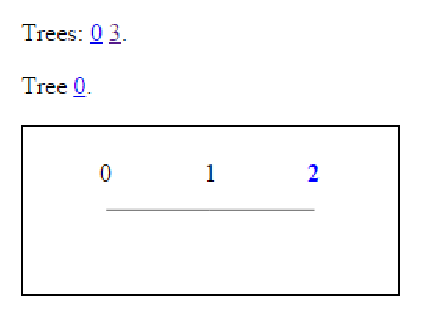
\includegraphics[scale=0.8]{ns_search_tree}
\caption[Needham-Schroeder search tree]{Search tree diagram for the
  initiator point of view in \texttt{ns.xhtml}}
\label{fig:ns init search tree}
\end{figure}

The search tree diagrams the steps in the search.  Each skeleton in
the entire graph file has a \index{label} label, a number starting
from 0.  The number associated with a tree is the label number of the
input skeleton.  The left edge of the search graph is the root of the tree:
in the case of Figure~\ref{fig:ns init search tree}, the graph does
not look very tree-like because the analysis doesn't branch.  The
numbers in the graph are the \index{label}labels of the skeletons
considered by {\cpsa} during its analysis, and clicking on a number
will direct the browser to display the corresponding skeleton.

The process by which {\cpsa} analyzes a skeleton is the repeated use
of an operation called the \index{cohort}\emph{cohort}, which takes an
input skeleton and produces a set of more refined skeletons that cover
all the possible executions the input skeleton covered.  The
relationship between a parent skeleton and a child is that a child is
included in the cohort calculated with the parent as an input.

\index{search tree}\index{search tree!colors} Numbers are normally
displayed in black, but may also be displayed in other colors.  Blue
numbers represent \emph{realized} skeletons, that is, skeletons that
may represent an actual execution.\footnote{Note that while realized
  skeletons already represent complete executions, \cpsa does further
  analysis once a realized skeleton is reached in order to
  \emph{generalize} that skeleton as much as possible.  A skeleton
  that is both realized and cannot be further generalized is a
  \index{shape}\emph{shape}.  See page \pageref{anchor:generalization}
  for more detail on generalization.}  Red numbers represent
\emph{dead} skeletons, that is, skeletons that represent partial
executions that are not part of any actual execution -- in other
words, impossible scenarios.

\index{skeleton!realized}\index{skeleton!dead} Numbers may occur in
the tree more than once, because it is possible that {\cpsa} will
discover a particular skeleton through more than one branch of the
analysis.  Green, italicized numbers represent skeletons present in
more than one branch that are not dead skeletons, while orange
italicized numbers represent dead skeletons present in more than one
branch.

Each skeleton starts with a line that indicates its label
(\texttt{item}) and the labels of its parent ((\texttt{parent}), if
any) and its children ((\texttt{child}), if any) See Fig.~\ref{fig:ns
  skel1}) The parent and child numbers link to those skeletons, while
the ``item'' number links back to the tree this skeleton is part of.

\begin{figure}
\centering
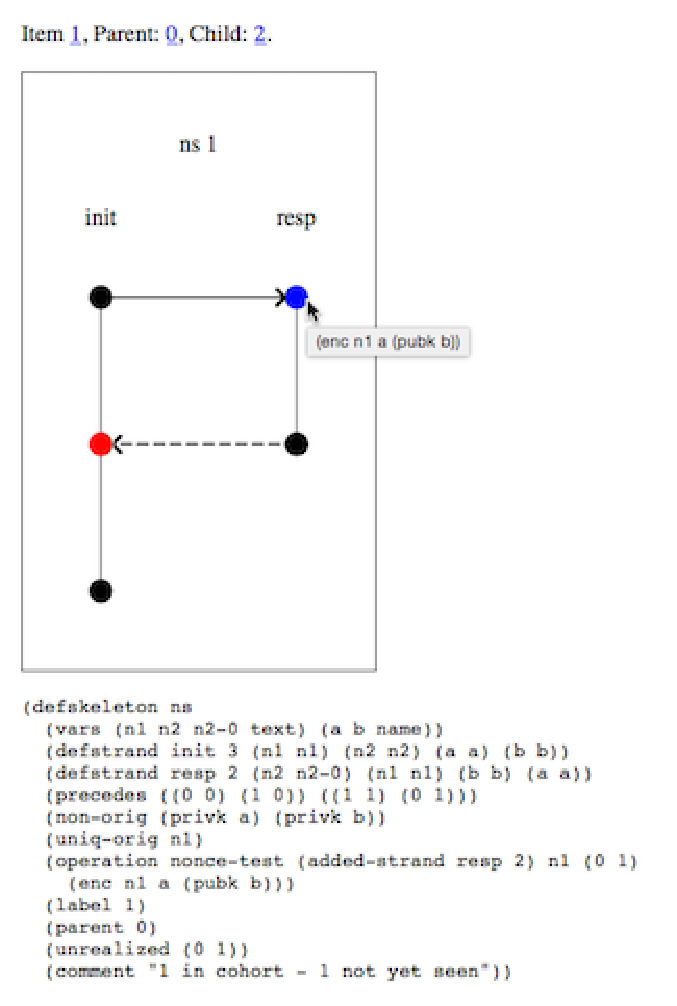
\includegraphics[height=7in]{ns_skel1_cursor}
\caption[Needham-Schroeder skeleton]{Skeleton from the initiator point
  of view in \texttt{ns.xhtml}}
\label{fig:ns skel1}
\end{figure}

Below the diagram is a \texttt{defskeleton} that fully describes the
skeleton.  This text is fully compatible with {\cpsa} input and can be
used as a skeleton input for analysis with this protocol, although
some of the fields in it are added by {\cpsa} and would be ignored
during input, for instance, the \texttt{label} and \texttt{parent}
fields.

The diagram shows the skeleton as a graph.  Strands are columns,
ordered from top to bottom.  The nodes in the graph are events,
normally transmissions or receptions of messages.  Nodes may be blue,
red, or black; a black node represents a transmission, while blue and
red nodes represent receptions.  A blue node represents an explainable
reception while a red node represents an unexplainable one.  The
left-most strands in a skeleton are normally the strands from the
input \texttt{defskeleton}.

\index{tooltip!skeleton node} The user may hover their mouse cursor
over any node and will see a display of the S-expression describing
the message at that event (see Figure~\ref{fig:ns skel1}). Here, if we
hover over the red node (as shown) we will see that this is an event where the
initiator receives the message $\enc{n1, n2}{K_a}$.  This occurs after
two transmissions: the first event in the init strand and the second
in the resp strand.  Those two transmissions are $\enc{n1, a}{K_b}$
and $\enc{n1, n2_0}{K_a}$.  Neither transmission is the expected
message, but sometimes a reception can be explained even if no regular
node sends the exact message.  Here, it is a question of what the
adversary can build given the messages available.  In this skeleton
there are \texttt{non-orig} or \texttt{uniq-orig} assumptions about
$n1, SK_a$, and $SK_b$, so since both messages are encrypted under
keys for which we have a secrecy assumption on the decryption key, the
adversary is unable to decrypt them.  The adversary is also unable to
build the required message: although the adversary is allowed access
to $n2$ and $K_a$ (since there are no restrictions on those), the
adversary does not have access to $n1$.  Hence, this node is
unexplainable.

Arrows in the diagram represent basic orderings in the skeleton;
arrows go from earlier events to later events.  An arrow is solid when
it goes from an event transmitting a message to one receiving the same
message. So the blue node in this example is obviously explained
because the exact message was transmitted by the initiator,
specifically, at the first node in the initiator strand.  The arrow
ending at the red node is dashed because the messages do not agree,
but it still represents that in this skeleton the second node of the
responder strand occurs before the second node of the initiator strand.

\section{Interpreting shapes}

Next, we turn our attention to Figure~\ref{fig:ns init shape}, which
is the one shape found by {\cpsa} during the search on the initiator
point of view.

\begin{figure}
\centering
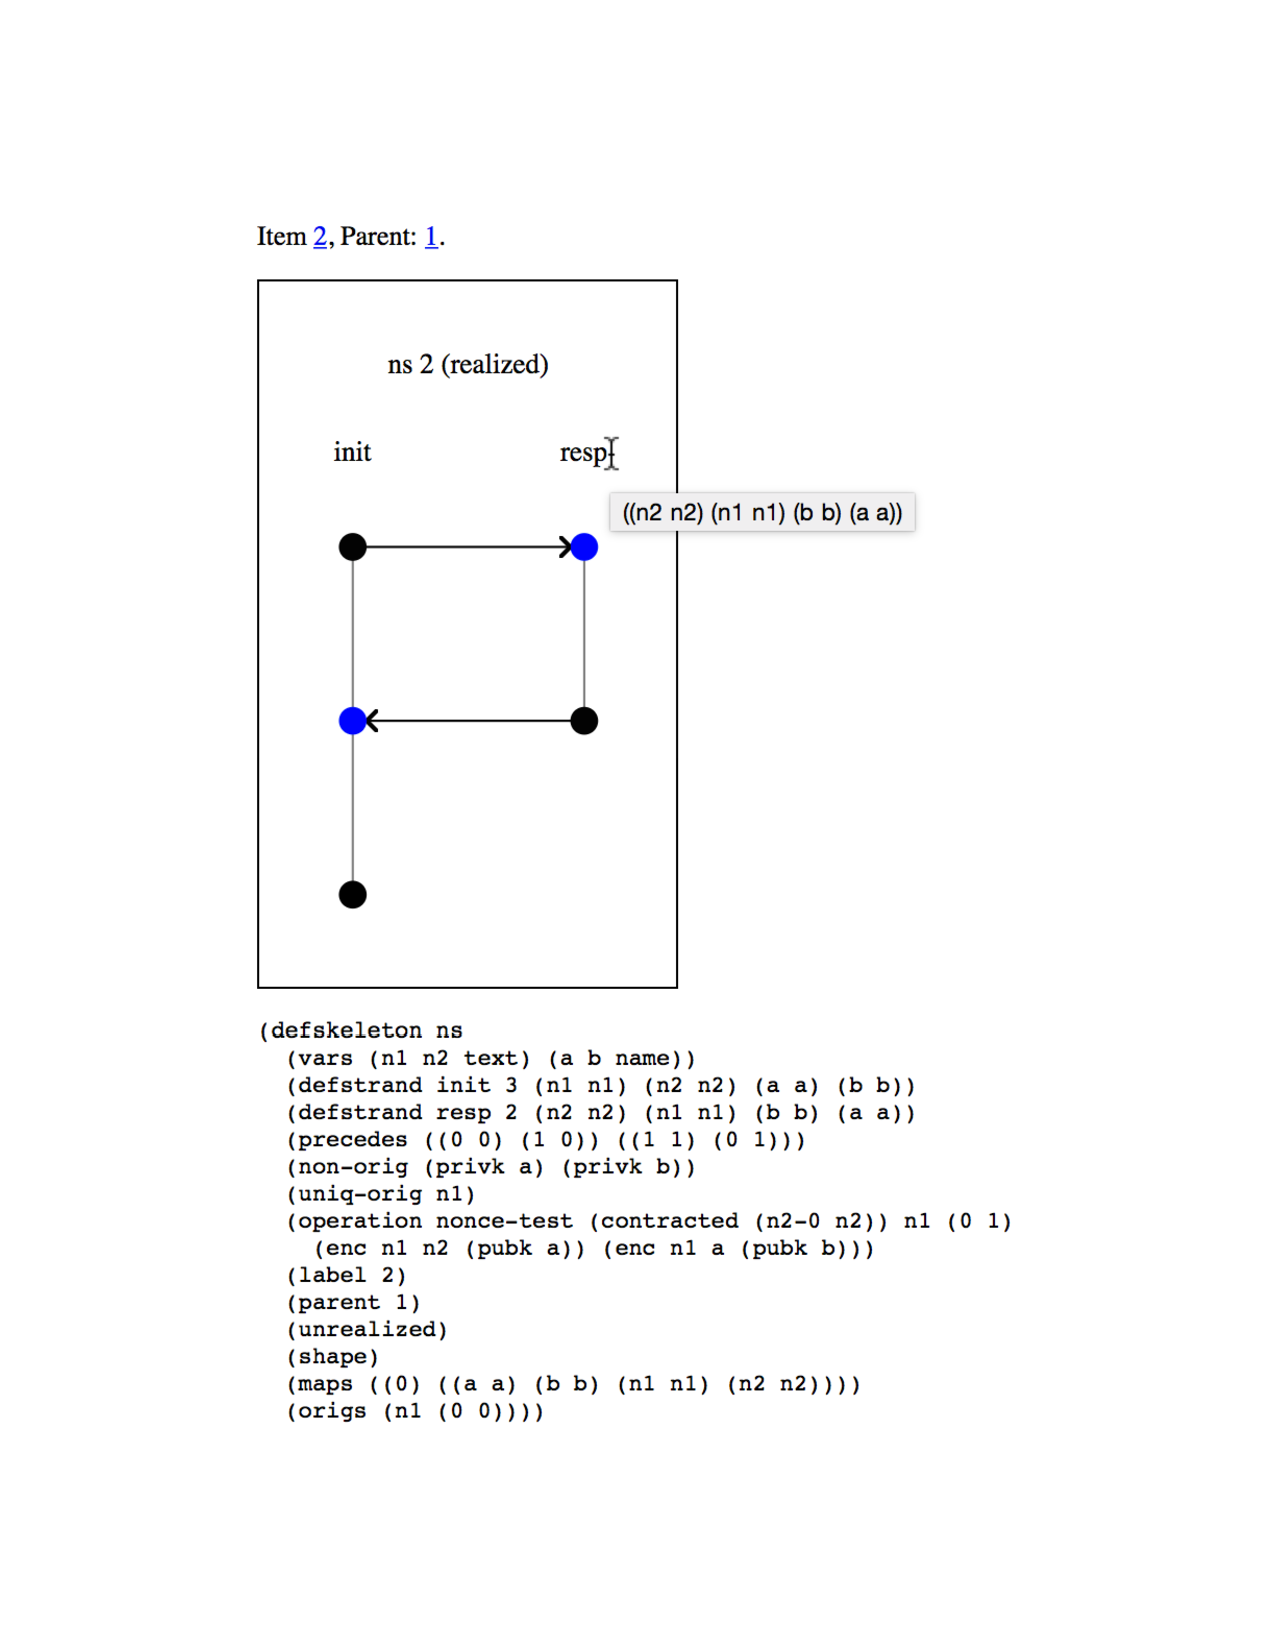
\includegraphics[height=7in]{ns_skel2_cursor}
\caption[NS shape, initiator point of view]{The only shape from the
  initiator point of view (\texttt{ns.xhtml})}
\label{fig:ns init shape}
\end{figure}

Before we get into detail on what is contained in this skeleton, note
the graph.  All the arrows are solid, and there are arrows everywhere
we expect them to be.  This describes a message being sent by an
initiator and received, unaltered, by a responder, who then sends a
message that is received, again unaltered, by the same initiator, who
then sends a message.

\index{tooltip!instance} The user can hover their mouse cursor over
the name of the role at the top of a strand in the skeleton diagram to
see the variable assignment used in that instance.  Here, hovering
over both the instances indicates that they are in agreement about the
values of $n1, n2, a$, and $b$: that is, the initiator's internal
value for each variable is the same as the responder's internal value
for the variable of the same name.

It may seem slightly odd that the initiator sends a message in its
third node that is not received by anyone, but we know that in general
it need not be received.  The adversary completely controls the network,
so it does not have to deliver that message.

\paragraph{The responder's point of view.}
The shape found during the search on the \emph{responder's} point of
view, however, includes something unusual.  See Figure~\ref{fig:ns
  resp shape}.

\begin{figure}
\centering
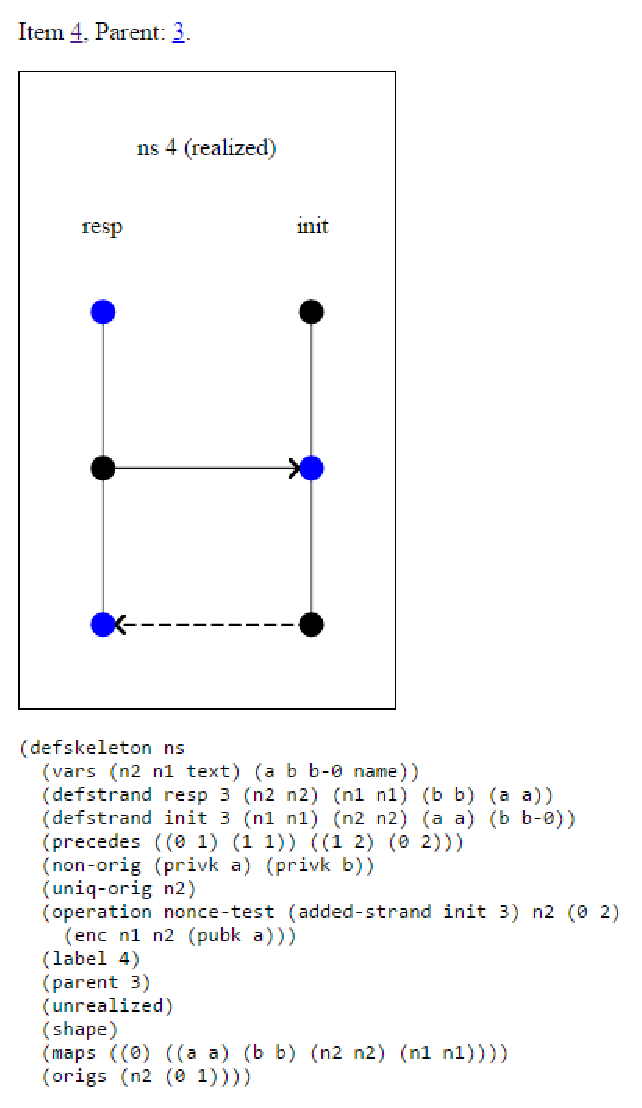
\includegraphics[scale=0.9]{ns_skel4}
\caption[NS shape for responder point of view]{The only shape in the
  responder point of view search in \texttt{ns.xhtml}}
\label{fig:ns resp shape}
\end{figure}

The graph of this shape should look less like expected behavior.  Two
things look odd, even at first glance.  Most noticeable is the dashed
arrow from the third initiator node to the third responder node.
Also, there's the fact that there is a blue node (the one in the top
left) that does not have any arrow coming in.

Inspection of the instances in this shape reveals that the initiator
and responder agree on all the values except for $b$.  This explains
the dashed arrow: the initiator sends $\enc{n2}{K_{b_0}}$ but the
responder receives $\enc{n2}{K_b}$; these messages are not the same,
which is why the arrow is not solid.  As for how the responder could
receive the proper value, note that we only assumed $SK_a$ and $SK_b$
are secure, but we did not assume $SK_{b_0}$ was secure.  It would have
been hard to do so, since $b0$ is a value we know nothing about from
the initiator's point of view. The initiator's transmission of
$\enc{n2}{K_{b_0}}$ thus does not protect $n2$ from decryption, so an
attacker could have created the responder's received message by
encrypting $n2$ under $K_b$.

The lack of an incoming arrow for the responder's first node can be
explained because of the lack of any assumption about the value $n1$.
The value $n1$ is the initiator's nonce, but this analysis does not
assume that an initiator, if present, will choose their nonce
properly.  So $n1$ could actually be a value already chosen by the
adversary, and the message $\enc{n1,a}{K_b}$ can be constructed and
delivered to the responder before the initiator even starts.

The fact that the initiator and responder do not agree on $b$ is an
interesting feature of this protocol.  We know from the initiator's
point of view that the initiator $a$, when they have completed their
execution, can infer that $b$ has taken part in the responder role
with $a$, and that they agree on both nonces.

The responder's point of view leads to less information.  The
responder $b$ knows that $a$ has taken part in the initiator role, but
does not know that $a$ intended to initate communication with $b$.
This lets us conclude that the Needham-Schroeder protocol provides
less than an ideal level of authentication.

\index{Lowe attack}
\index{Needham-Schroeder-Lowe protocol}
\begin{exercise}
  The attack described above was first identified by Gavin
  Lowe~\cite{Lowe96a}, who also proposed a fix, namely, to have the
  second message in the Needham-Schroeder protocol include the name
  $b$ of the responder.

Make a copy of the Needham-Schroeder input file and modify the
protocol so that the second message (in both roles) includes a $b$.
Run the analysis again and graph it.  You should observe that the
disagreement on $b$ from the responder's point of view is no longer
possible, and that the initiator's point of view is still good.
\end{exercise}

\section{Blanchet's simple example protocol}
\label{sec:blanchet}

\index{Blanchet protocol} \index{examples!Blanchet} Next we turn our
attention to a second protocol, which will help build the reader's
experience with {\cpsa} and also introduce some additional features.
This protocol is due to Bruno Blanchet, and has a flaw introduced by
design for the purpose of discussing protocol analysis.  In this
protocol there are again two participants: an initiator and a
responder.  However, in this protocol, we do not use names, just
public keys.  Specifically, one party has a public signing key ($a$),
while the other has a public encryption key ($b$).

The protocol is as follows, informally:

\begin{itemize}

\item The initiator chooses a fresh, random session key $s$, signs it
  with their private signing key (corresponding to the public key
  $a$), and encrypts it with the responder's public key $b$ and sends
  the result to the responder.

\item The responder receives and decrypts such a message, confirms the
  signature, and then encrypts a piece of data $d$ under $s$ and sends
  this back to the initiator.
\end{itemize}

The file \texttt{blanchet.scm} in the examples directory contains
Blanchet's simple example protocol described above.  See
Figure~\ref{fig:blanchet defprotocol} for the protocol declaration.

\begin{figure}
\centering
\begin{tabular}{l}
\verb|(defprotocol blanchet basic|\\
\verb|  (defrole init|\\
\verb|    (vars (a b akey) (s skey) (d data))|\\
\verb|    (trace (send (enc (enc s (invk a)) b))|\\
\verb|           (recv (enc d s)))|\\
\verb|    (uniq-orig s))|\\
\verb|  (defrole resp|\\
\verb|    (vars (a b akey) (s skey) (d data))|\\
\verb|    (trace (recv (enc (enc s (invk a)) b))|\\
\verb|           (send (enc d s)))|\\
\verb|    (uniq-orig d)))|
\end{tabular}
\caption{The Blanchet simple example protocol}
\label{fig:blanchet defprotocol}
\end{figure}

\ttindex{akey} \ttindex{skey} \ttindex{data} There are several
elements of this protocol input that are new.  First of all, the
Needham-Schroeder protocol used only two types: \texttt{name} and
\texttt{text}, while this protocol uses three new types.  The
\texttt{data} type is for simple values, much like \texttt{text}.  In
fact, the two types are interchangeable, but both are available for
cases where an analyst may wish to describe a protocol in which two
types of simple values exist that cannot be confused for each other.

The \texttt{akey} and \texttt{skey} types are for keys, specifically,
asymmetric and symmetric keys, respectively.  The \texttt{invk}
function symbol maps an asymmetric key to its inverse.

\index{signatures} Note that we use \texttt{(enc s (invk a))} to
represent the digital signature.  A digital signature in the {\cpsa}
message algebra is represented as an encryption under the signature
key.

\index{role declarations} A third feature is the presence of a
delcaration such as \texttt{(uniq-orig s)} within a
\texttt{defrole}.  Like the \texttt{uniq-orig} declaration that can
appear in a skeleton, this declaration indicates that the value
contained inside is freshly chosen.  When this declaration appears in
the role, however, the assumption is that the value is freshly chosen
by \emph{every} honest participant in the protocol who plays that
role.  Declarations present in a role are inherited by every skeleton
with an instance of that role.  See Chapter~\ref{ch:declarations} for
more on the declarations supported by \cpsa.

\begin{exercise}
Make a variant of the Needham-Schroeder protocol in which the
freshness of each party's nonce is assumed via a \texttt{uniq-orig}
declaration in the protocol role.  Run the analysis from each
participant's point of view.  What differs in the shapes, and why?
(There should be one difference that's noticeable in the graph of one
of the shapes.)
\end{exercise}

\begin{exercise}
Make a variant of the Needham-Schroeder protocol in which the secrecy
of each party's partner's private key is assumed via a
\texttt{non-orig} declaration in the protocol role.  Run the analysis
from each participant's point of view.

You should observe that the authentication failure is no longer
present in the shape from the analysis of the responder's viewpoint.
What conclusion can you draw about this declaration?  Did we fix the
protocol?  If not, why does the analysis seem to contain no flaws?
\end{exercise}

The \texttt{blanchet.scm} file contains four inputs to the analysis.
The first and second are just the points of view of each participant,
under typical assumptions.  But the third and fourth contain another
new element.  See Figure~\ref{fig:blanchet pov3-4} for these two
inputs.

\begin{figure}
\centering
\begin{tabular}{l}
\verb|(defskeleton blanchet|\\
\verb|  (vars (a b akey) (s skey) (d data))|\\
\verb|  (defstrand init 2 (a a) (b b) (s s) (d d))|\\
\verb|  (deflistener d)|\\
\verb|  (non-orig (invk b)))|\\\\
\verb|(defskeleton blanchet|\\
\verb|  (vars (a b akey) (s skey) (d data))|\\
\verb|  (defstrand resp 2 (a a) (b b) (s s) (d d))|\\
\verb|  (deflistener d)|\\
\verb|  (non-orig (invk a) (invk b)))|\\\\
\end{tabular}
\caption{Blanchet points of view}
\label{fig:blanchet pov3-4}
\end{figure}

\ttindex{deflistener}\index{listener} These two inputs are prepared to
ask a confidentiality question: specifically, is the value $d$ exposed
to the adversary?  A \emph{listener} is a pseudo-role that is
considered part of all protocols by {\cpsa}.  That role consists of
receiving some arbitrary message and then sending that same message.
Listeners can show up in {\cpsa} analyses, in order to handle a case
where a certain value is learnable, so that the rest of the case
breakdown can assume that value is not learnable.

\index{skeleton!dead}
In this protocol, the secret data $d$ remains private in the
initiator's point of view.  Figure~\ref{fig:blanchet tree 6} shows the
search tree for the point of view in which the initiator completes the
protocol and in which there is a listener for the same $d$ value the
initiator hears.  The fact that all the numbers are red here indicates
that all the skeletons in the search are ``dead'', meaning that they are
inconsistent with any actual executions.  In other words, there are no
executions in which $d$ is revealed given our assumption that the private
decryption key of $b$ is not compromised.

However, $d$ does not remain private in the responder's point of view.
Figure~\ref{fig:blanchet skel 13} shows the graph of a shape for the
point of view in which the responder completes the protocol and in
which there is a listener for the $d$ value the responder sends.  Note
that although $d$ is encrypted under $s$, and $s$ is freshly chosen by
an initiator, the shape shows that $s$ can leak.  We are not
guaranteed that the initiator and responder agree on $b$.  Therefore,
the initiator may have sent $s$ encrypted with $b_0$, and since the
private key corresponding to $b_0$ is not necessarily secret, $s$ may
leak.

\begin{figure}
\centering
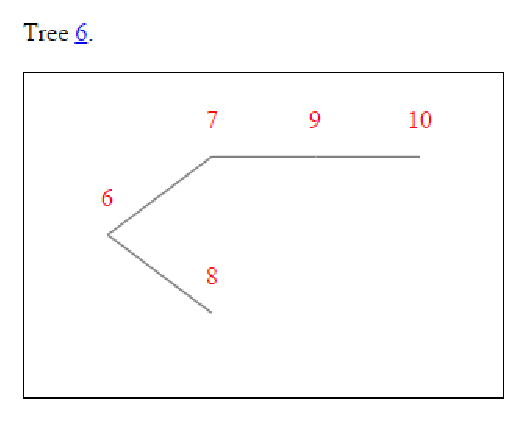
\includegraphics{blanchet_tree6}
\caption[Blanchet privacy search tree]{The search tree for the privacy
  of $d$ in the initiator's point of view in \texttt{blanchet.xhtml}}
\label{fig:blanchet tree 6}
\end{figure}

\begin{figure}
\centering
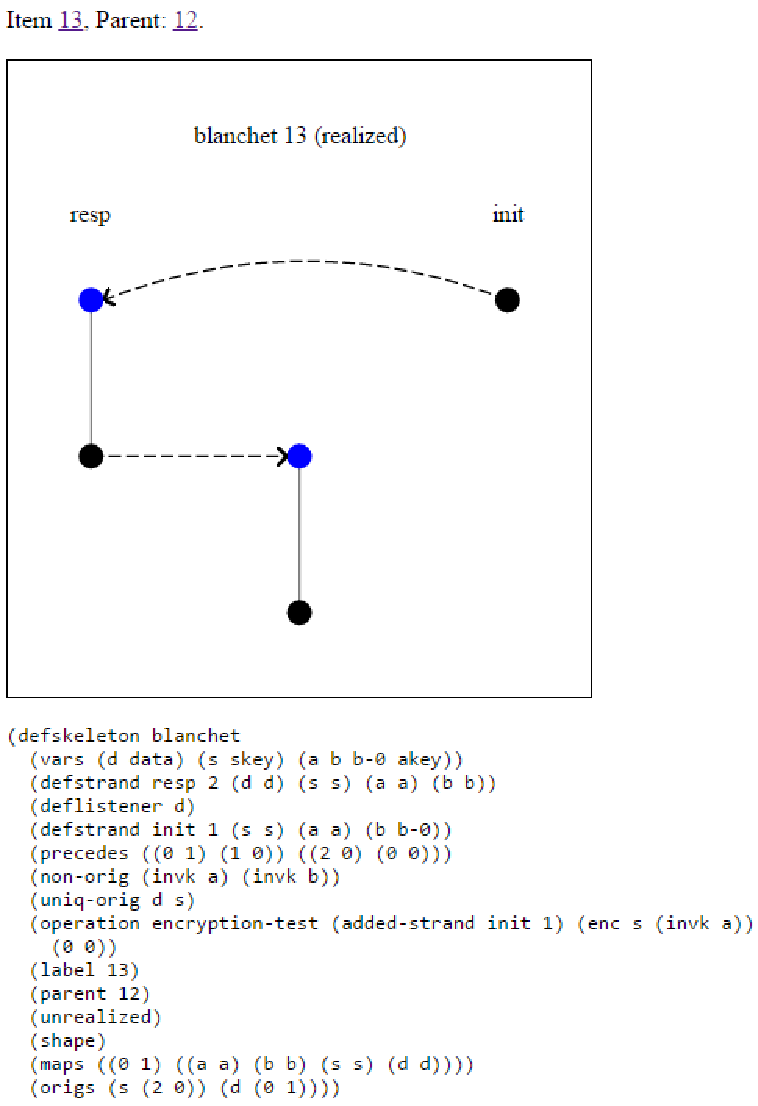
\includegraphics[scale=0.9]{blanchet_skel13}
\caption[Blanchet shape for responder's point of view]{The only shape
  in the analysis for the responder's point of view with a listener
  for $d$ in \texttt{blanchet.xhtml}.  The second strand, with no role
  name, is the listener. }
\label{fig:blanchet skel 13}
\end{figure}

The \texttt{blanchet.scm} file also contains a second protocol with
the name \texttt{blanchet-corrected} in which the flaw that allows $d$
to be learned in the responder's point of view is eliminated.

\begin{exercise}
  Modify the Blanchet protocol to add a role that is identical to the
  initiator role, except that $s$ is not declared \texttt{uniq-orig}.
  What impact does this have on the analyses?
\end{exercise}

\begin{exercise}
  If you modify the Blanchet protocol to instead add a role that is
  identical to the responder role, except that $d$ is not declared
  \texttt{uniq-orig}, what impact do you believe this will have on the
  analyses?  Make a prediction, then check your prediction.
\end{exercise}

\begin{exercise}
\label{ex:noroledecls_blanchet}
Try modifying the Blanchet protocol, removing the \texttt{uniq-orig}
declarations from the two roles.  Replace the \texttt{defskeleton}s in
the input file with the point of view skeletons for the un-corrected
version of the Blanchet protocol from \texttt{blanchet.xhtml}; these
skeletons will explicitly include declarations that would be inherited
but were lost due to the removal of the role declaration.
\end{exercise}

\iffalse{
    % This exercise illustrates the CPSA 3 restriction on uniq-orig
    % assumptions for values that do not have a point of origination
    % in the skeleton already.  This restriction no longer exists in
    % CPSA 4 -- it is not needed -- so we have edited out the
    % exploration 
    
    \begin{exercise}
      Starting from your modified version of the Blanchet protocol from
      Exercise~\ref{ex:noroledecls_blanchet}, add a \texttt{uniq-orig} declaration
      on $s$ to the point of view with a responder instance and a listener for $d$.

      This should produce an error message, because {\cpsa} expects that for
      every value declared to be uniquely originating, that value originates
      at some point in the skeleton.  When only the responder's strand and
      the listener are present, $s$ does not originate; it is received by
      the responder before being used in an outgoing message, and it does
      not occur on the listener strand at all.

      Now add a \texttt{defstrand} adding an instance of an initiator
      (height 1), using the same $s$, and declare $s$ to be uniquely
      originating.  Check that the resulting shape is the same attack shape
      as in the unmodified \texttt{blanchet.xhtml}.
    \end{exercise}}
\fi 

%  See Section~\ref{sec:role_decls2} for more about how role
%  declarations work.

%%% Local Variables:
%%% mode: latex
%%% TeX-master: "cpsa4manual"
%%% End:
